\subsection{Execution and results}
%erkl�ren, !was! wir machen, !warum! wir das machen und mit welchem ziel
%(wichtig) pr�zize erkl�ren, wie bei dem versuch vorgegangen und was gemacht wurde
In this section the execution and the results will be presented.

\subsection{Identification of the lines and measurement of the absorption}

In this measurement all 39 theoretical expected lines in the spectrum should be measured. At first the pressure for this measurement has to be around 10$^{-1}$mbar and constant. The pressure during the measurement was at 9,8$ \cdot$ 10$^{-2}$. The measurement started at the 28GHz, because the peaks in that range are bigger then the ones at the beginning of the spectrum. For the measurement of the peaks the wave meter was used. The dip from the wave meter was positioned right on the dip of the NH$_3$ and the frequence was the take from the wave meter. Then the oscilloscope was used to determine the hight of the peaks. For that the dip of the wave meter was scrolled out of the visible spectrum on the oscilloscope. Then the to bars on the oscilloscope were used to determine the size of the dip. 

With the size of the dip the absolute absorption coefficient can be calculated. The absolute absorption coefficient is calculated by formula \ref{equ:alpha}. U$_0$ was not know so the coefficients where normed to the size of the the 3 3 peak, so $\alpha_{rel_{3,3}}$ = 1. All measured Date can be find in table \ref{tab:data_39_1},\ref{tab:data_39_2}.

\begin{align}
\label{equ:alpha}
\alpha_{rel} = \frac{10}{l} \cdot ln(1- \frac{U_a}{U_0})
\end{align}

\begin{table}[H]
\begin{tabular}{c|c}
l & lenght of the wave guide, 5m in this buildup \\ 
U$_a$ & the intensity without any absorption \\ 
U$_0$ & the intensity of the measured peak \\ 
\end{tabular} 
\end{table}

\begin{figure}[H]
\centering
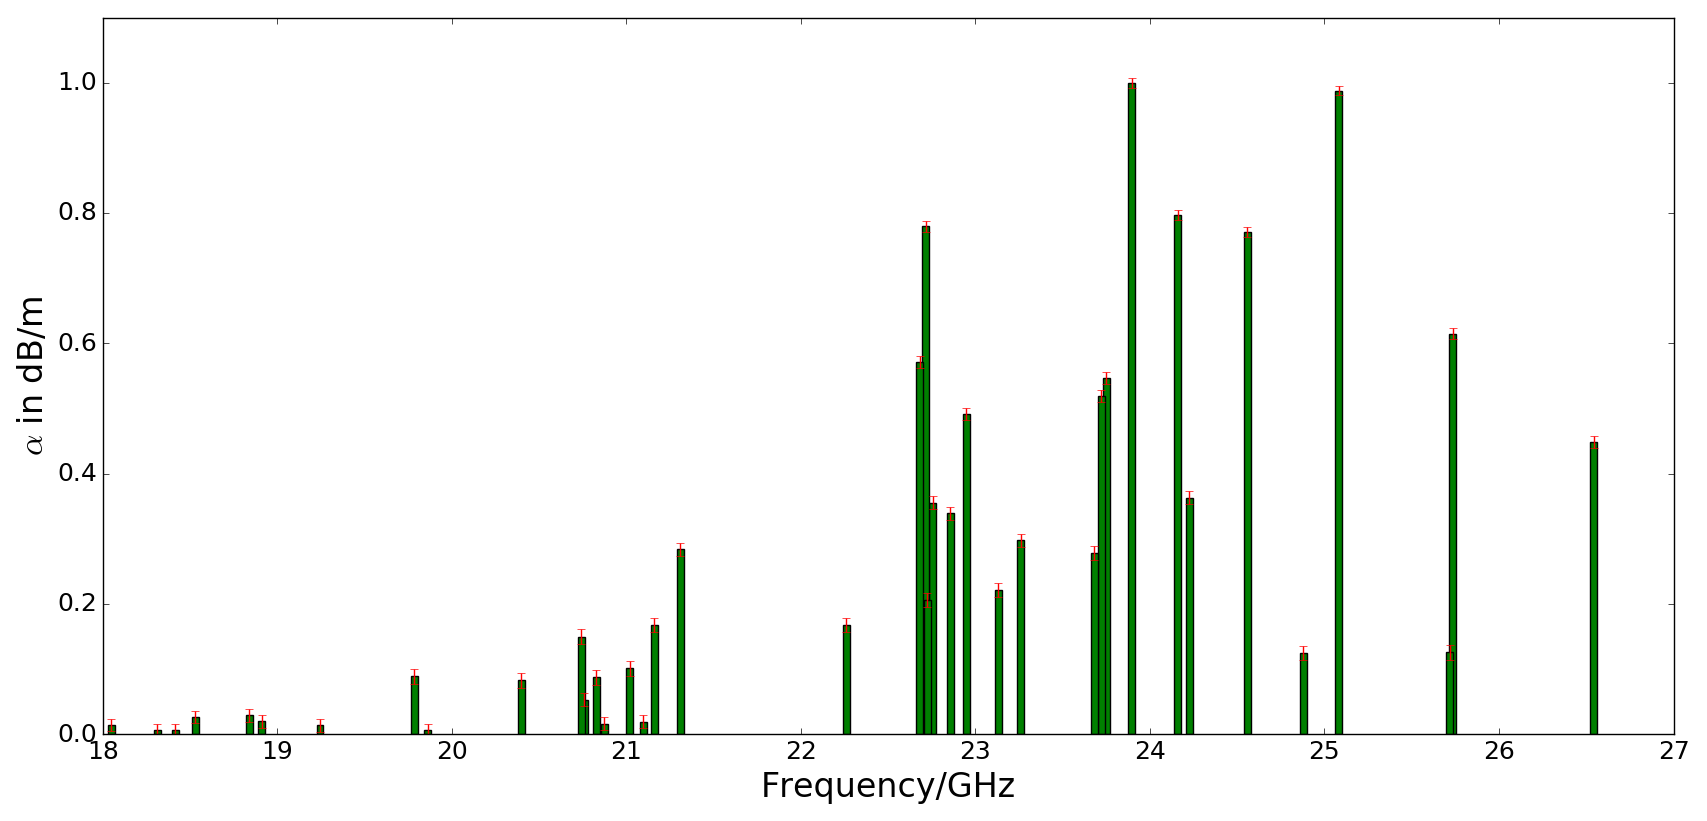
\includegraphics[scale = 0.39]{alpha.png}
\caption{The plot shows the relative absorption coefficient, the coefficient was calculated with formula \ref{equ:alpha}. The errors where taken from the uncertainty of the listing}
\label{fig:alpha}
\end{figure}





\subsection{Hyperfinestructure}
In this section the quadrupole moment of the NH$_3$ will be calculated using the hyperfine structure. Three peaks where measured for the calculation but only for 2 of them the fit for the five peaks converged. The process of fitting and analyzing the data is done as example for the 3 3 peak, for the 4 4 peak the same procedure was used.

At first a calibration is done, because the oscilloscope can only measure the current depended on the time. For the calibration 3 peaks where created with the wave meter, so the frequency is known for them. The peaks are fitted with a Lorentz distribution, witch is given in equation \ref{equ:lorentz}. 

\begin{align}
\label{equ:lorentz}
f(x) = \frac{A}{\pi} \cdot \left( \frac{\sigma}{(x-\mu)^2 + \sigma^2} \right)
\end{align}

To get a better fit result, first the underground was fitted and subtracted from the data. For the fit of the underground a polynomial of sixth degree was used. An example can be seen in figure \ref{fig:hf_untergrund}.

\begin{figure}[H]
\centering
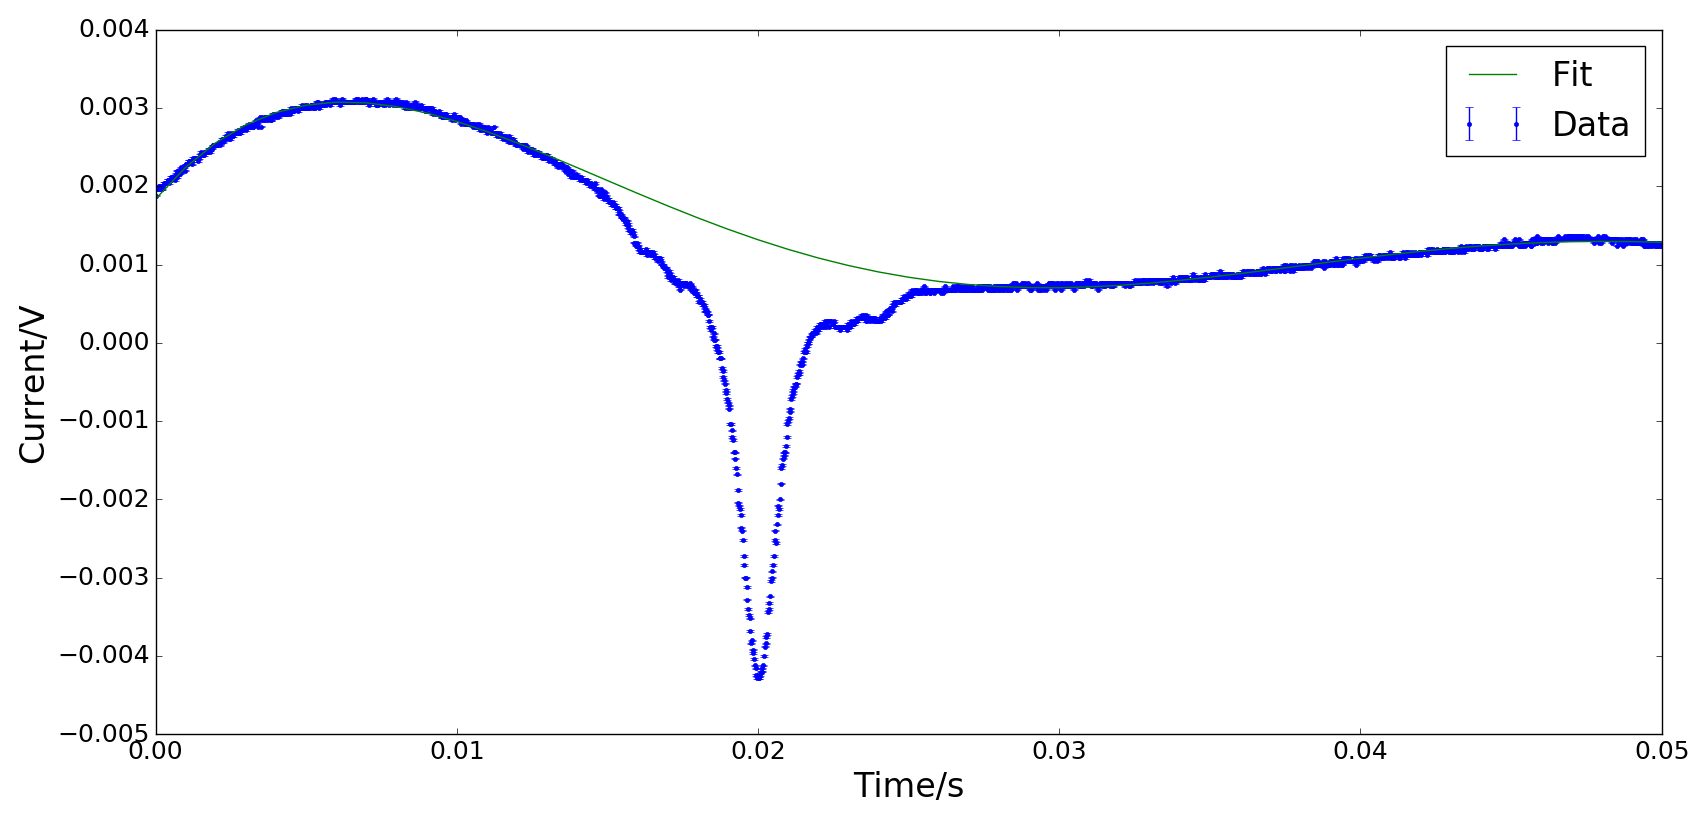
\includegraphics[scale = 0.39]{untergrund_hf.png}
\caption{The plot of the 3 3 data and the fitted underground}
\label{fig:hf_untergrund} 
\end{figure}

The data without the underground and a peak for the calibration can be seen in figure \ref{fig:hf_untergrund_fit}. The values of the centers of the Lorentz distribution obtained with the fits are given in table \ref{tab:claib_6_6}.

\begin{figure}[H]
\centering
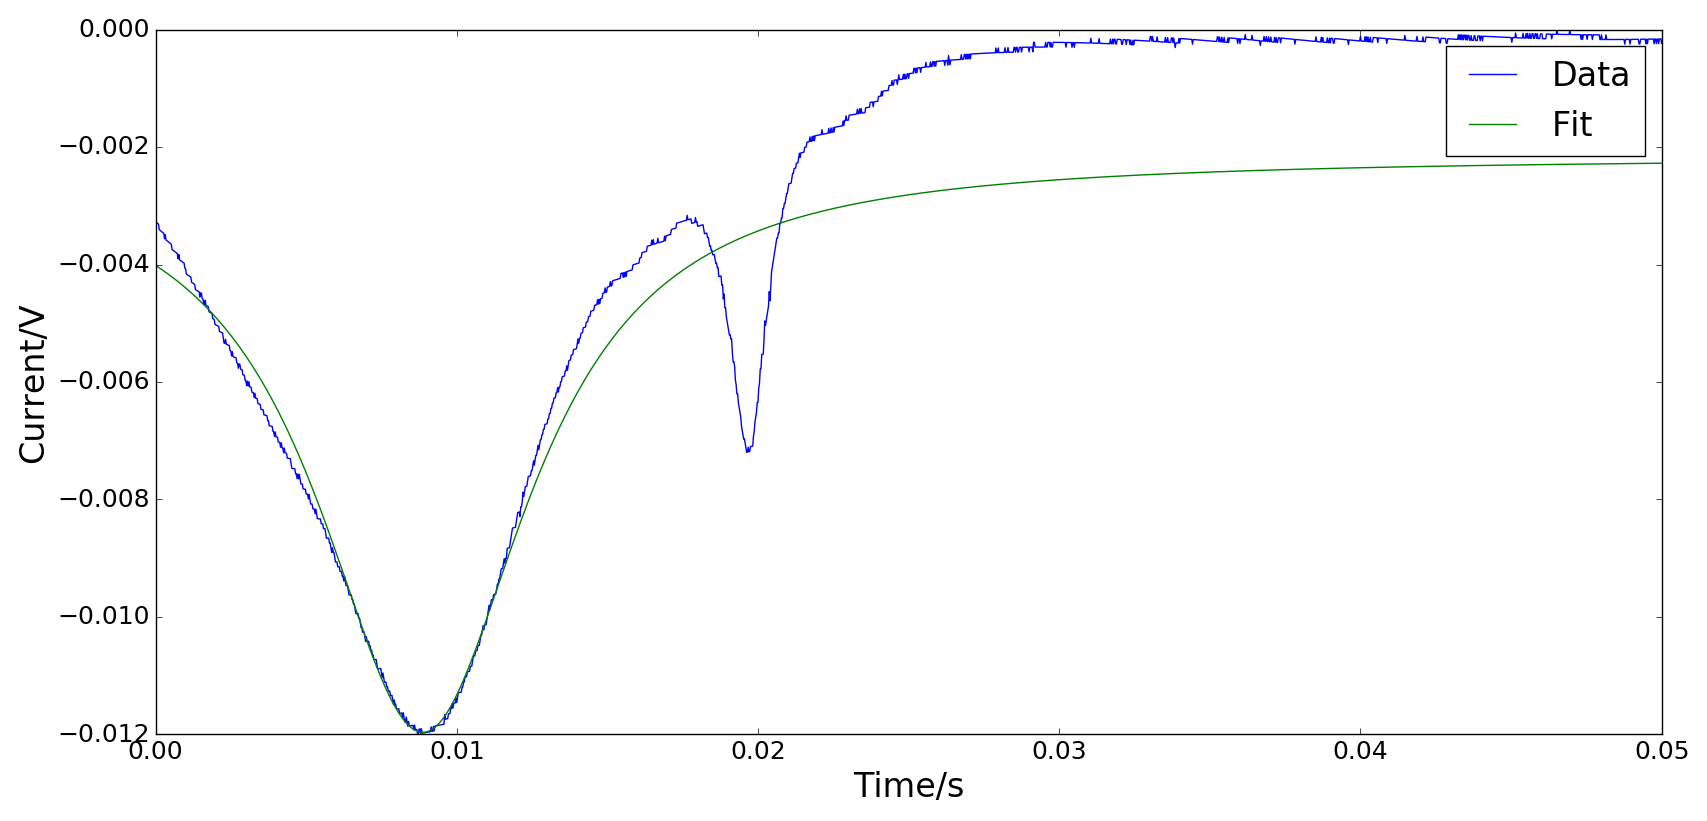
\includegraphics[scale = 0.39]{hf_kalib_peak_1.png}
\caption{The plot of the 3 3 data for the calibration, without underground}
\label{fig:hf_untergrund_fit} 
\end{figure}

\begin{table}[H]
\centering
\caption{Fitparameters for the peaks used for the calibration of the 6 6 peak.}
\label{tab:claib_6_6}
\begin{tabular}{c|c|c}
Peak & Center/ms & $\chi_{red}^2$ \\ \hline
1 & 0.8874(4) & 0.53 \\ 
2 & 0.0248(5) & 0.82 \\ 
3 & 0.0406(3) & 1.12 \\ 
\end{tabular} 
\end{table}

The linear fit for the dependency between time and frequency is given in figure \ref{fig:hf_lin_fit} the parameters can be found in table \ref{tab:claib_6_6_lin}.

\begin{figure}[H]
\centering
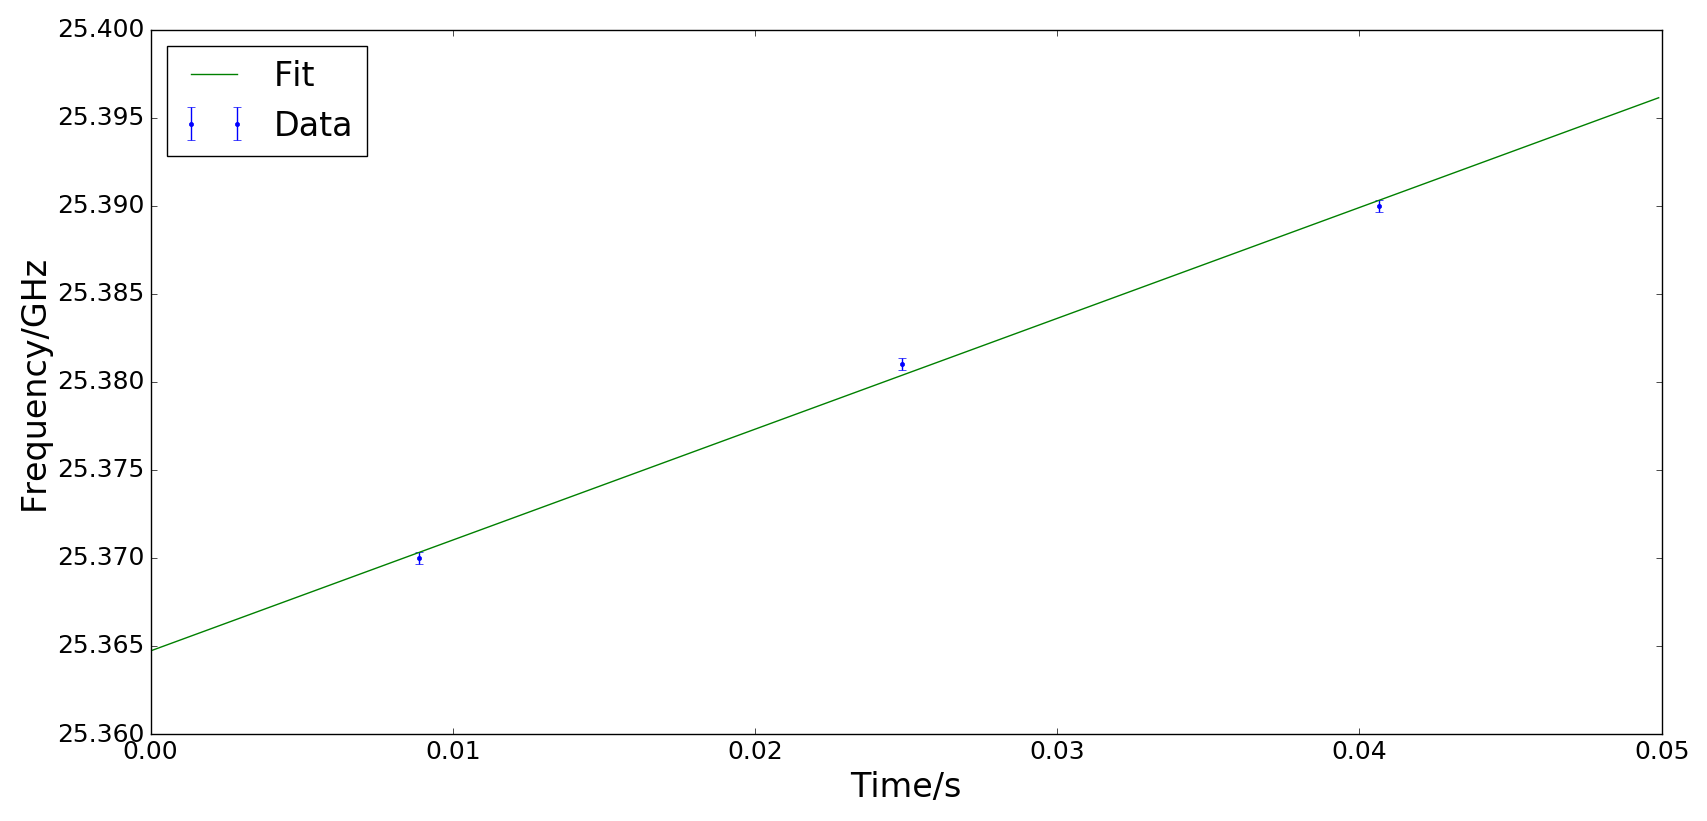
\includegraphics[scale = 0.39]{hf_kalib_lin_1.png}
\caption{Linear fit for the calibration}
\label{fig:hf_lin_fit} 
\end{figure}

\begin{table}[H]
\centering
\caption{Fitparameters for the calibration of the 6 6 peak.}
\label{tab:claib_6_6_lin}
\begin{tabular}{c|c|c}
Peak & Center/ms & $\chi_{red}^2$ \\ \hline
1 & 0.8874(4) & 0.53 \\ 
2 & 0.0248(5) & 0.82 \\ 
3 & 0.0406(3) & 1.12 \\ 
\end{tabular} 
\end{table}

The fit for the 3 3 peak with the hyperfine structure can be seen in figure \ref{fig:hf_6_6}, the parameters of the fit are in the appendix \ref{sec:hf_anhang}.

\begin{figure}[H]
\centering
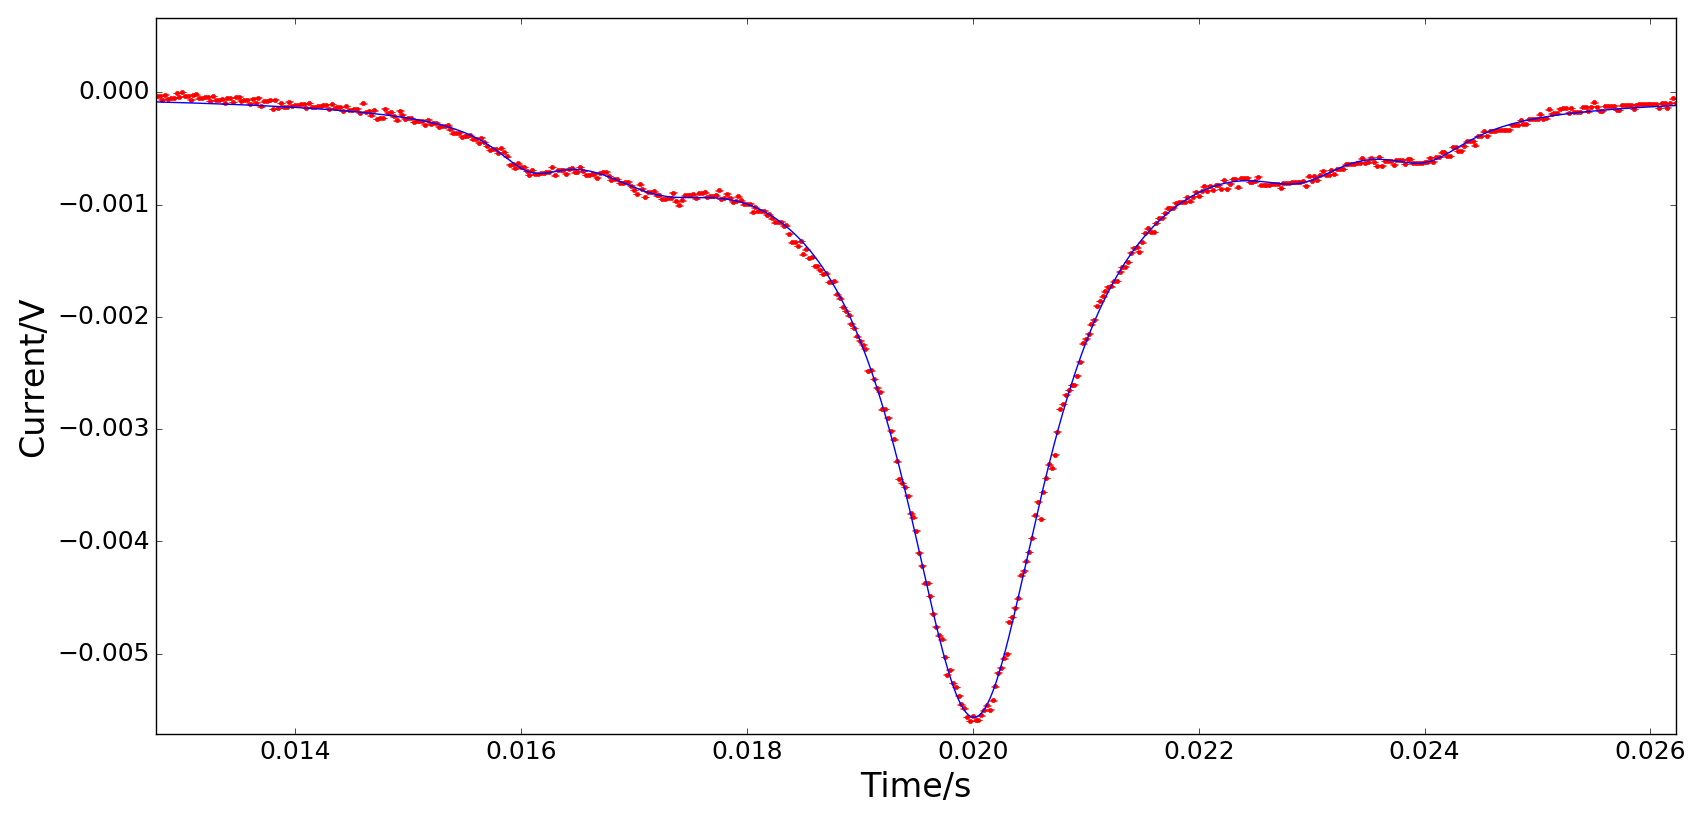
\includegraphics[scale = 0.39]{hf_6_6.png}
\caption{Linear fit for the calibration}
\label{fig:hf_6_6} 
\end{figure}

From the positions of the peaks the quadrupole moment of can be calculated. For the calculation the distance between the main peak and the side peaks is needed. The distances between the main peak and the side peaks in given in table \ref{tab:qudru_fit_data}.

\begin{table}[H]
\centering
\caption{Distances of the side peaks to the main peak}
\label{tab:qudru_fit_data}
\begin{tabular}{c|c|c|c}
Peak & Side & Distance of the outer/MHz & Distance of the inner/MHz \\ \hline 
3 3  & Right & 2.52(4) & 1.82(1) \\ 
3 3 & Left & 2.47(3)  & 1.76(4) \\ 
4 4 & Right & 2.55(3) & 2.068(9) \\ 
4 4  & Left & 2.72(4) & 2.10(2)  \\ 
\end{tabular} 
\end{table}


With equation \ref{eqn:Hyperfine} the quadrupole moment can be calculated, $\beta$ is taken from \cite{examenarbeit}. In table \ref{tab:quad_data} the calculated values for the quadrupole moment are given.

\begin{table}[H]
\centering
\caption{Calculated quadropol moments}
\label{tab:quad_data}
\begin{tabular}{c|c|c|c}
Peak & Side & Inner peak/MHz & Outer peak/MHz \\ \hline 
3 3 & Right & 5.29(5) & 5.82(1)  \\ 
3 3 & Left & 5.65(2) & 5.91(3) \\ 
4 4 & Right & 4.54(3) & 4.40(2) \\ 
4 4 & Left & 4.33(4) & 4.25(3) \\ 
\end{tabular} 
\end{table}

The mean of the values in table \ref{tab:quad_data} is 5.02(9), the theoretical value is 4.14 \cite{hf_book}.



\subsection{Dependency between pressure and line width of the 3 3 peak}
In this section the dependency between the pressure and the line width will be examined. The 3 3 Peak was chosen, because it was was the biggest one. For the measurement the pressure is increased in steps and the spectrum is measured. The line broadening is given by equation \ref{equ:broadening}.

\begin{align}
\label{equ:broadening}
\Delta\nu = \sqrt{\frac{273}{T}} \cdot p \cdot \Delta
\end{align}

\begin{table}[H]
\begin{tabular}{c|l}
$\Delta \nu$ & line broadening at a temperature of 273K \\ 
T  & room temperature \\ 
p & pressure \\
$\Delta$ & specific to the gas, for NH$_3$ $\Delta$ = 29 $\frac{Mhz}{mmHg}$ \\ 
\end{tabular} 
\end{table}

For the calculation of $\Delta$ a calibration of the data is needed, because the oscilloscope only gives a time-volt dependency. For the calibration the centers of the three peaks with a know wave frequency are used and fitted with a linear model. The Peaks are fitted with a Lorentz distribution, see equation \ref{equ:lorentz}. The fit parameters for the calibration are in table \ref{tab:pressure_fit}. The Fit and the data can be seen in figure \ref{fig:druck_fit}.

\begin{table}[H]
\centering
\caption{Fit parameters for the three peaks for the calibration}
\label{tab:pressure_fit}
\begin{tabular}{c|c|c}
Peak & Value & $\chi_{red}^2$ \\ \hline 
1 & 0.0410(7) & 0.93 \\ 
2 & 0.0269(8) & 1.23 \\ 
3 & 0.0110(5) & 1.12 \\  
\end{tabular} 
\end{table}

\begin{figure}[H]
\centering
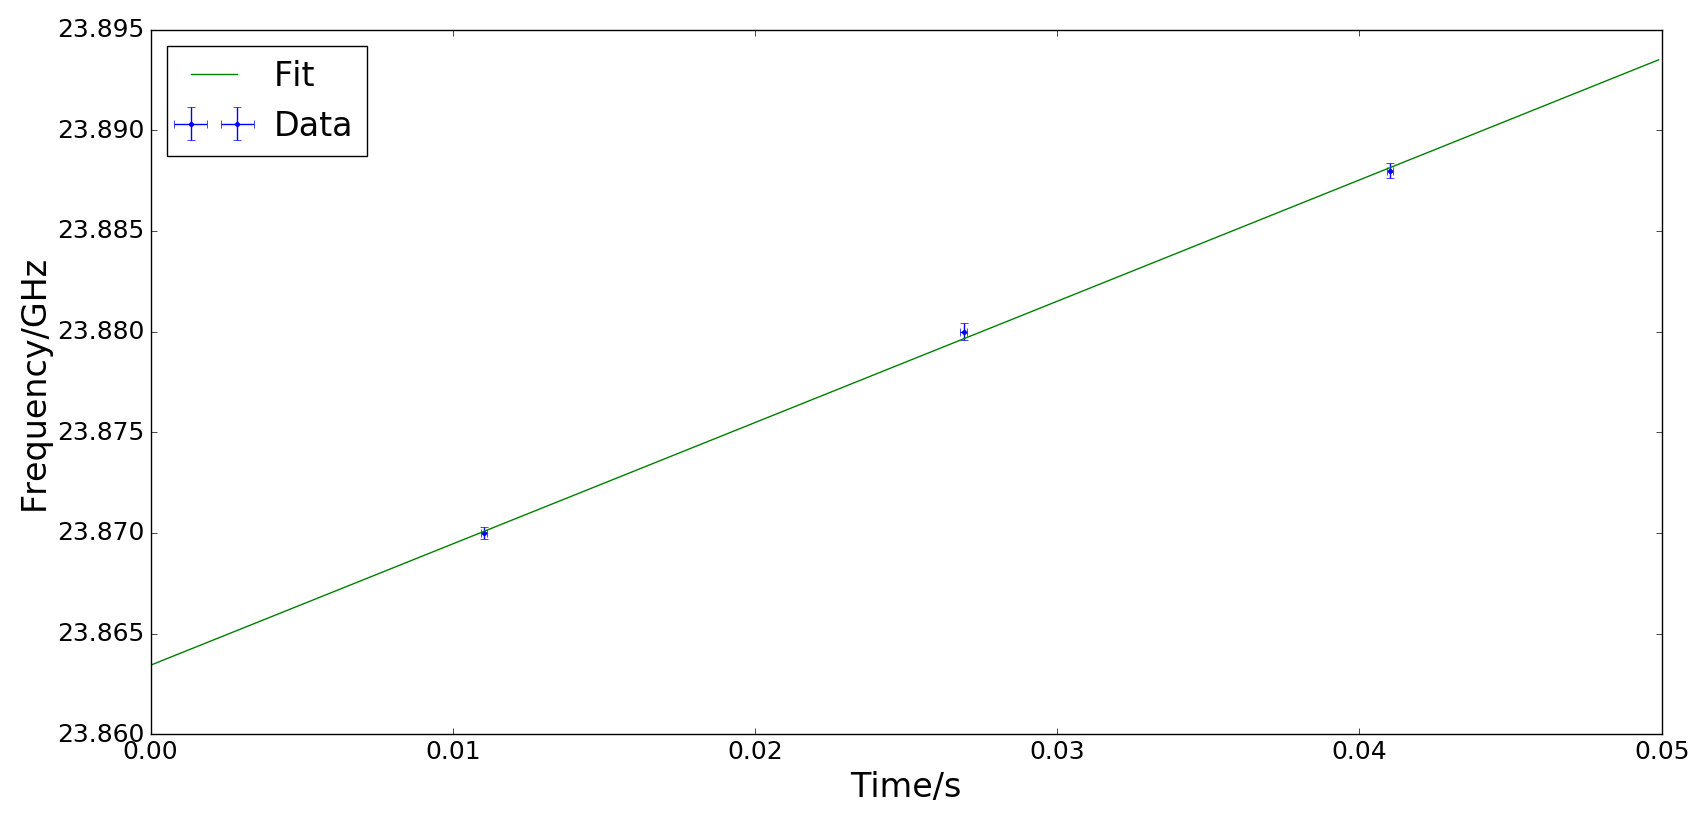
\includegraphics[scale = 0.39]{druck_kalib.png}
\caption{The plot shows the data and the linear fit for the calibration. The x-errors are so small, that they can barely be seen in the plot. The parameters of the fit can be found in table \ref{tab:pressure_fit_pars}}
\label{fig:druck_fit}
\end{figure}

\begin{table}[H]
\centering
\caption{Fit parameters for the calibration}
\label{tab:pressure_fit_pars}
\begin{tabular}{c|c}
Parameter & Value \\ \hline 
slope & 0.60(2) GHz/s \\ 
intercept & 23.863(4) GHz/s\\ 
$\chi^2_{red}$ & 0.98 \\  
\end{tabular} 
\end{table}

A plot of all the measured Peaks can be seen in figure \ref{fig:druck_alle}, the data from the measurement can be found in table \ref{tab:pressure_alle}. 

\begin{figure}[H]
\centering
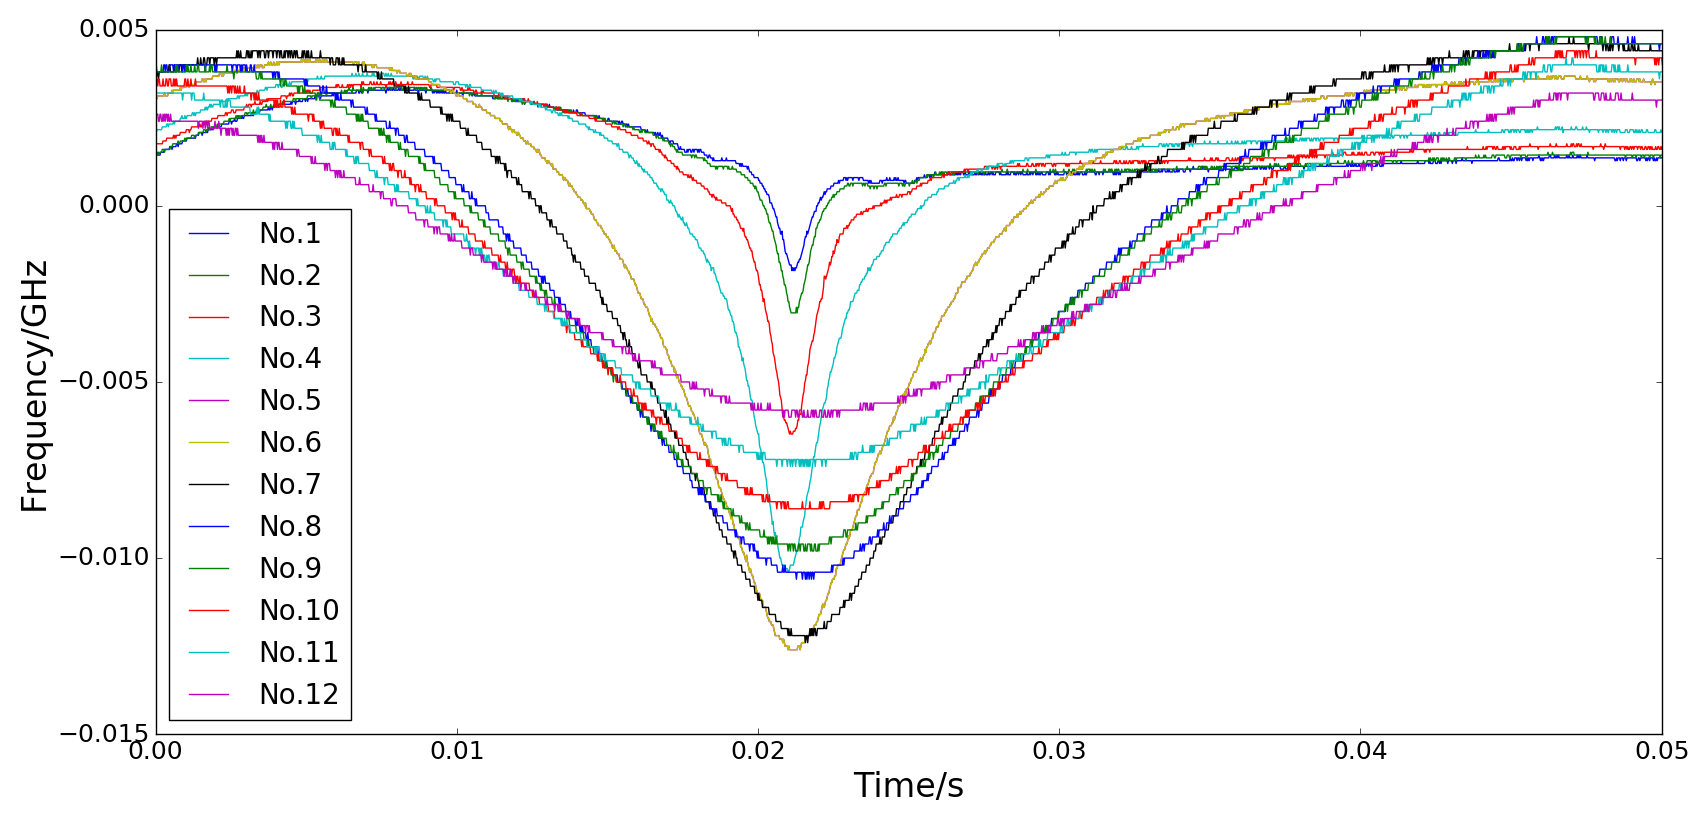
\includegraphics[scale = 0.39]{druck_alle.png}
\caption{The plot shows the 3 3 peak for different pressures, the pressures can be found in table \ref{tab:pressure_alle}.}
\label{fig:druck_alle}
\end{figure}

\begin{table}[H]
\centering
\caption{Pressures and line width for the measured peaks. The error one the pressure is 0.1mbar for every measurement.}
\label{tab:pressure_alle}
\begin{tabular}{c|c|c}
No. & Pressure/mbar & line width/ms \\ \hline
1 & 1.0 $\cdot 10^{-2}$ & 0.136(12) \\ 
2 & 2.6 $\cdot 10^{-2}$ & 0.139(16) \\ 
3 & 8.7 $\cdot 10^{-2}$ & 0.18(2) \\ 
4 & 1.5 $\cdot 10^{-1}$ & 0.31(2) \\ 
5 & 2.7 $\cdot 10^{-1}$ & 0.56(3) \\ 
6 & 3.8 $\cdot 10^{-1}$ & 0.82(5) \\ 
7 & 5.8 $\cdot 10^{-1}$ & 1.3(1) \\ 
8 & 9.3 $\cdot 10^{-1}$ & 1.7(2) \\ 
9 & 1.1 & 2.0(1) \\ 
10 & 1.3 & 2.3(3) \\ 
11 & 1.6 & 2.5(3) \\ 
12 & 2.0 & 2.8(2) \\ 
\end{tabular} 
\end{table}


In figure \ref{fig:beispiel_alle} an example for a fit of a peak and the underground estimation can be seen. The underground was fitted with a polynomial of 6 degree.


\begin{figure}[H]
\begin{subfigure}{.49\textwidth}
  \centering
  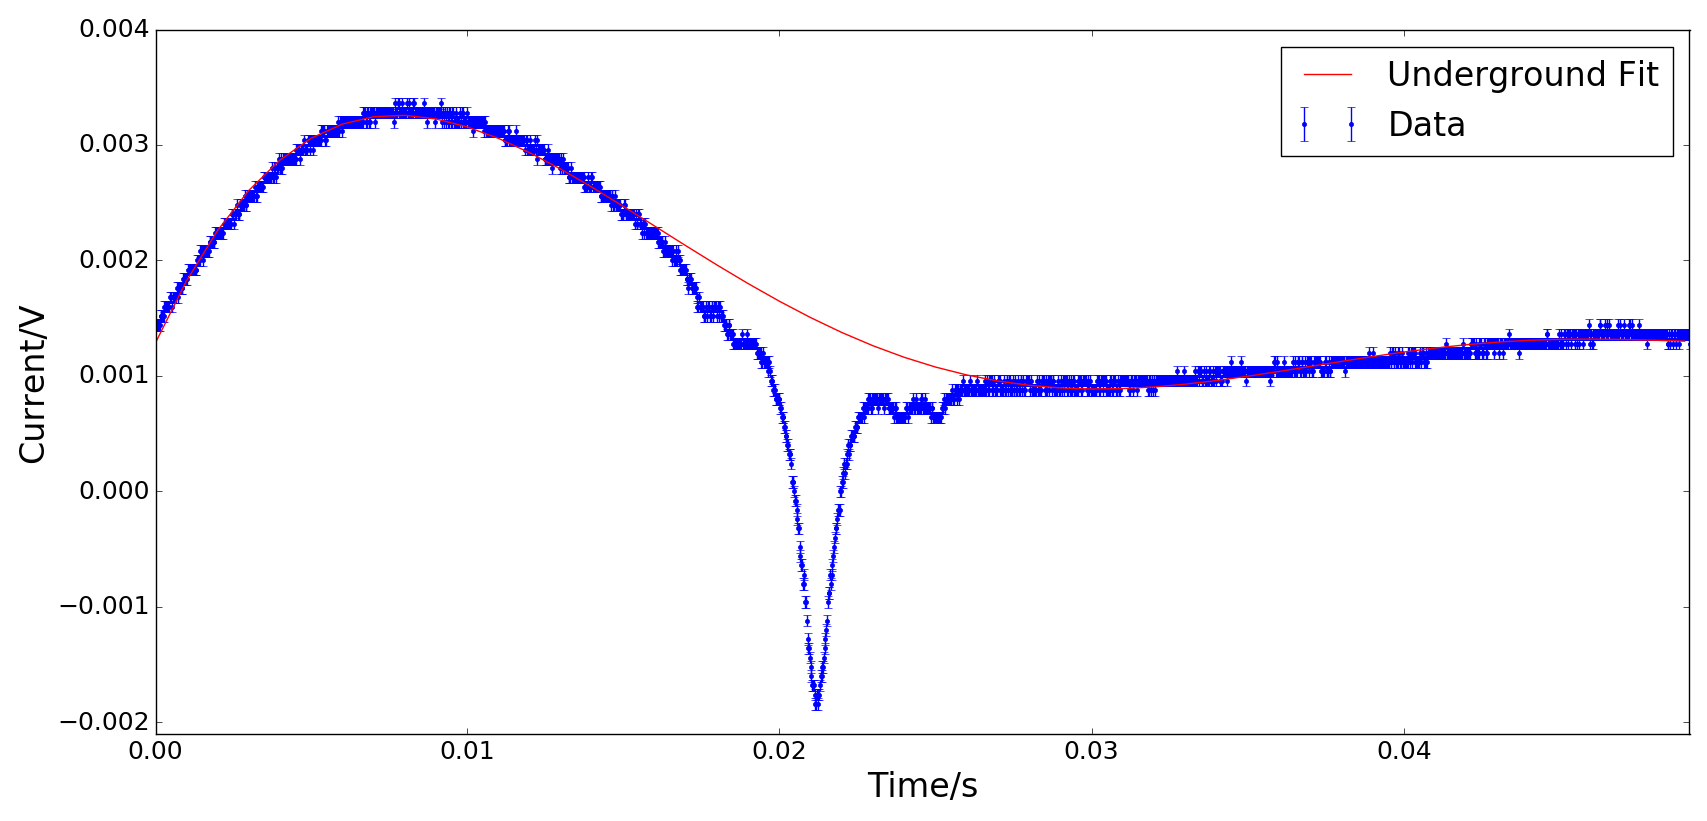
\includegraphics[width=\linewidth]{druck_beispiel_alle_untergrund.png}
  \caption{Plot of the 3 3 peak at a pressure of 1.0(1)$\cdot 10^{-2}$ with the underground fit.}
  \label{fig:beispiel_alle_1}
\end{subfigure}%
\begin{subfigure}{.49\textwidth}
  \centering
  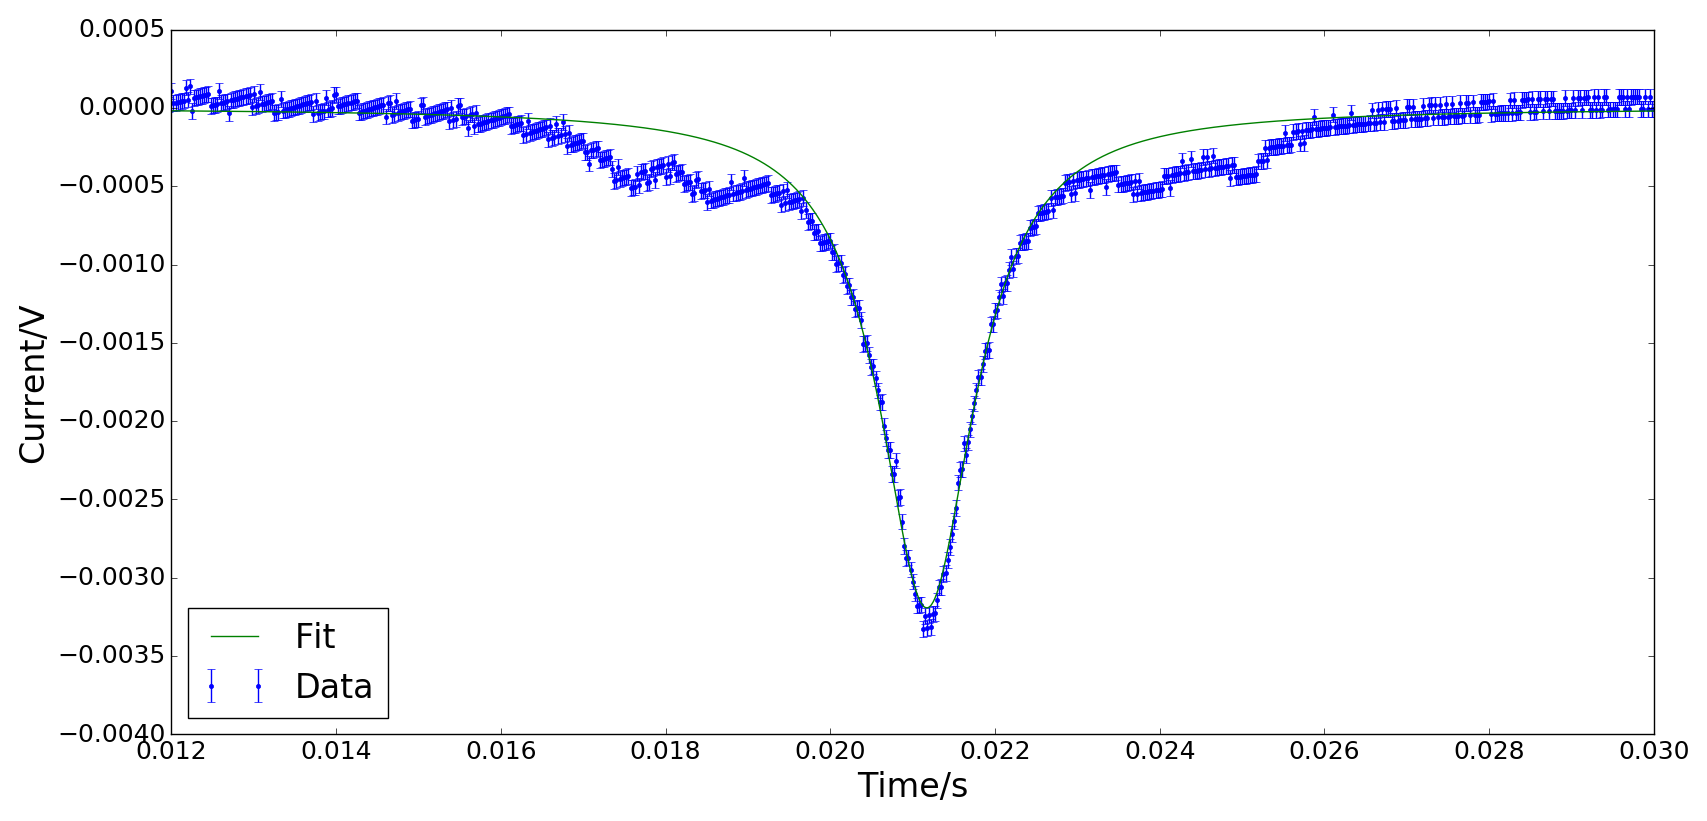
\includegraphics[width=\linewidth]{druck_beispiel_alle.png}
  \caption{Plot of the 3 3 peak at a pressure of 1.0(1)$\cdot 10^{-2}$ with removed underground.}
  \label{fig:beispiel_alle_2}
\end{subfigure}
\caption{Example plots of the peak fitting for the 3 3 peak at a pressure of 1.0(1)$\cdot 10^{-2}$ and underground estimation.}
\label{fig:beispiel_alle}
\end{figure}

The data from table \ref{tab:pressure_alle} is fitted with a linear model for estimation of $\Delta$. In figure \ref{fig:druck_lin_fit} the data and the fit is shown. The parameter of the fit are in table \ref{tab:pressure_lin_fit_pars}.

\begin{figure}[H]
\centering
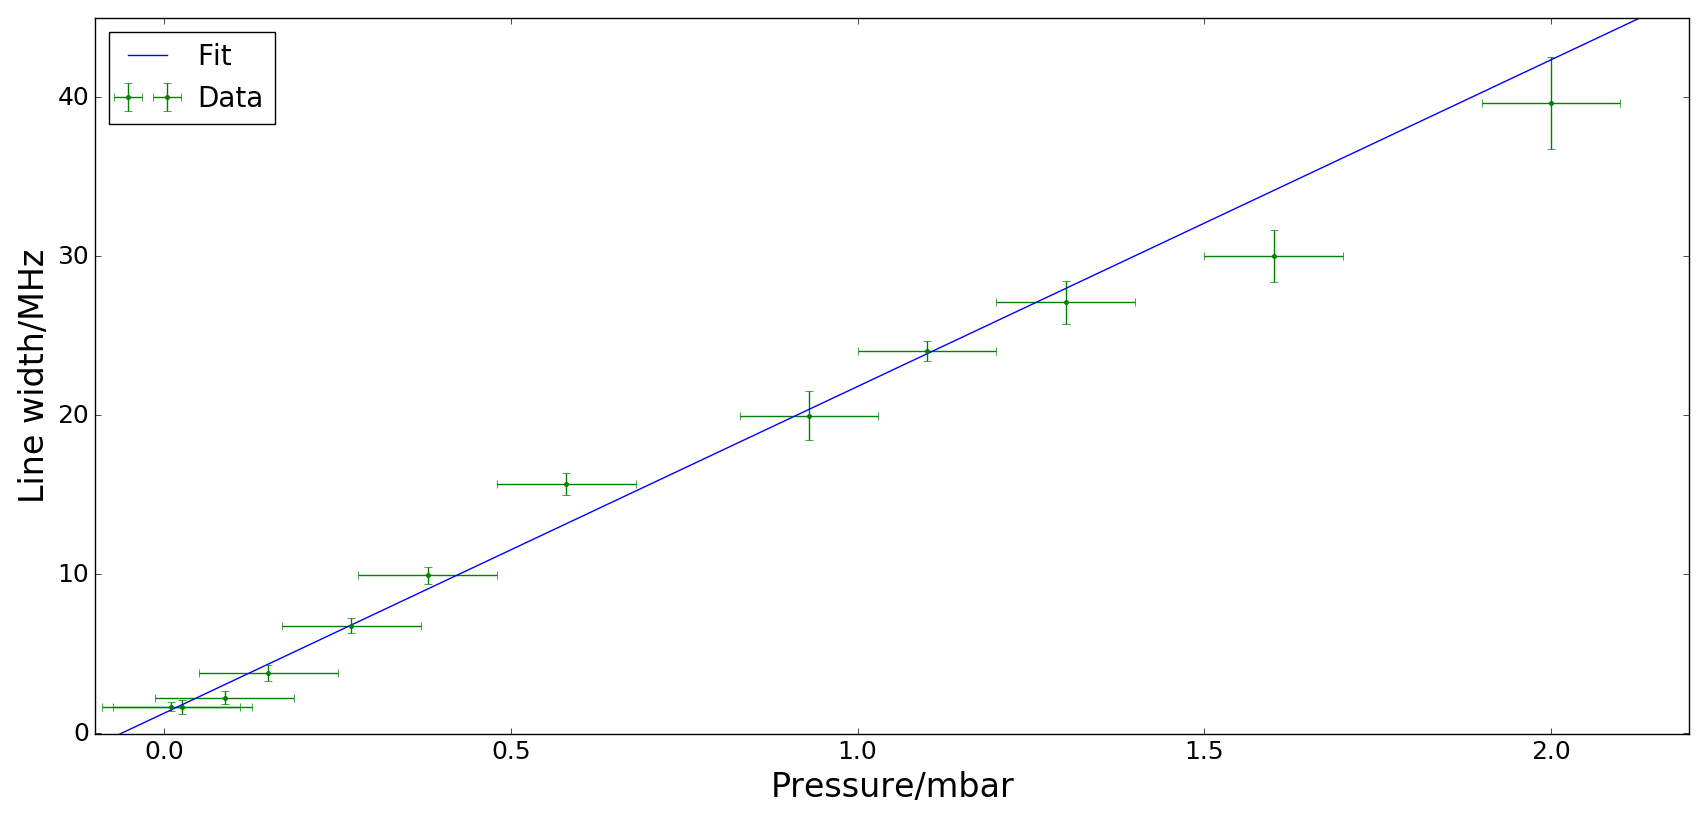
\includegraphics[scale = 0.39]{druck_hz_fit.png}
\caption{The plot shows the 3 3 peak for different pressures, the pressures can be found in table \ref{tab:pressure_lin_fit_pars}.}
\label{fig:druck_lin_fit}
\end{figure}

\begin{table}[H]
\centering
\caption{Fit parameters for the calibration}
\label{tab:pressure_lin_fit_pars}
\begin{tabular}{c|c}
Parameter & Value \\ \hline 
slope & 20(1) MHz/mbar\\ 
intercept & 1.2(2) MHz/mbar \\ 
$\chi^2_{red}$ & 2.91 \\  
\end{tabular} 
\end{table}

With equation \ref{equ:broadening} $\Delta$ can be calculated, where T=300K and $\Delta \nu$ = 20(1).

\begin{align*}
\Delta = 20(1) \sqrt{\frac{300}{273}} \frac{\text{MHz}}{\text{mbar}} = 21(1) \frac{\text{MHz}}{\text{mbar}} = 28(1) \frac{\text{MHz}}{\text{mmHg}}
\end{align*}

